\CVioBeginChapter{2}{II. Project Management Plan}
This chapter defines how the project was planned, coordinated, monitored, revised, and closed as an AI research project. The management plan is designed to support scientific validity as well as delivery discipline. It therefore covers not only schedule and task ownership, but also dataset integrity, experimental comparability, evidence traceability, mobile integration, document consistency, and the final submission constraint. The plan reflects the actual three-member working structure, the weekly supervision mechanism, and the transition from an initially classification-oriented scope to the final two-track classification and instance segmentation project.\par
The project differs from a conventional software-production project because the most important outputs are validated research evidence, reproducible model improvements, a defensible interpretation of results, and an integrated mobile demonstration. Progress is not measured only by completed code. A task is considered complete only when its inputs, configuration, output, evaluation, responsible owner, and relationship to the project objectives can be explained. This principle is applied throughout the team organization, WBS, risk controls, quality plan, change procedure, and Definition of Done presented in this chapter.\par
\section{Team Work}
\subsection{Team Structure and Roles}
The project team consists of one academic supervisor and three student members. The supervisor assigns weekly research tasks and reviews milestones. The project leader coordinates execution, deadlines, technical integration, reproducibility, and document delivery. After Session 3, responsibilities were separated into a classification track led by Tran Huu Nhan, an attention-based segmentation and mobile track led by Le Thi Huynh Nhu, and a dataset-labeling and Fourier-based segmentation track led by Nguyen Van Phong.\par
\begingroup
\CVioTableSetup
\begin{longtable}{|>{\centering\arraybackslash}p{2.65cm}|>{\centering\arraybackslash}p{1.95cm}|>{\centering\arraybackslash}p{2.39cm}|>{\centering\arraybackslash}p{6.72cm}|}
\caption{Team structure and roles}\\
\hline
\CVioPeachHeader\textbf{Member} & \textbf{Student ID} & \textbf{Role} & \textbf{Main responsibilities} \\ \hline
\endfirsthead
\caption[]{Team structure and roles (continued)}\\
\hline
\CVioPeachHeader\textbf{Member} & \textbf{Student ID} & \textbf{Role} & \textbf{Main responsibilities} \\ \hline
\endhead
\hline
\multicolumn{4}{r}{\footnotesize Continued on next page}\\
\endfoot
\hline
\endlastfoot
Nguyen Dinh Vinh & - & Supervisor & Weekly task assignment; research direction; milestone evaluation; academic feedback \\ \hline
Tran Huu Nhan & CE181655 & Project Leader & Coordination; YOLO26m-cls selection; ASL-LDAM; SimAM-DCFR; classification evaluation; reproducibility; paper/thesis integration; TFLite support \\ \hline
Le Thi Huynh Nhu & CA182007 & Member & Android requirements; UI/UX; Kotlin/Java; authentication; camera/gallery; TFLite; Firebase; admin dashboard; mask display; attention segmentation; documentation \\ \hline
Nguyen Van Phong & CE192081 & Member & Initial preprocessing; baseline benchmarking; single-annotator BG/WSSV masks; YOLO conversion; grouped split; leakage analysis; segmentation baselines; Fourier experiments; robustness; documentation \\ \hline
\end{longtable}
\endgroup
Table 2.1 preserves the complete member information while clarifying the technical ownership of each workstream. It also shows that the supervisor is responsible for academic direction rather than implementation, whereas the project leader is responsible for coordination and integration across all tracks.\par
Figure 2.1 visualizes the reporting and responsibility structure described in Table 2.1. The hierarchy places the supervisor above the project leader, followed by the two specialized member tracks and the shared final-delivery responsibilities.\par
\begin{figure}[tbp]
\centering
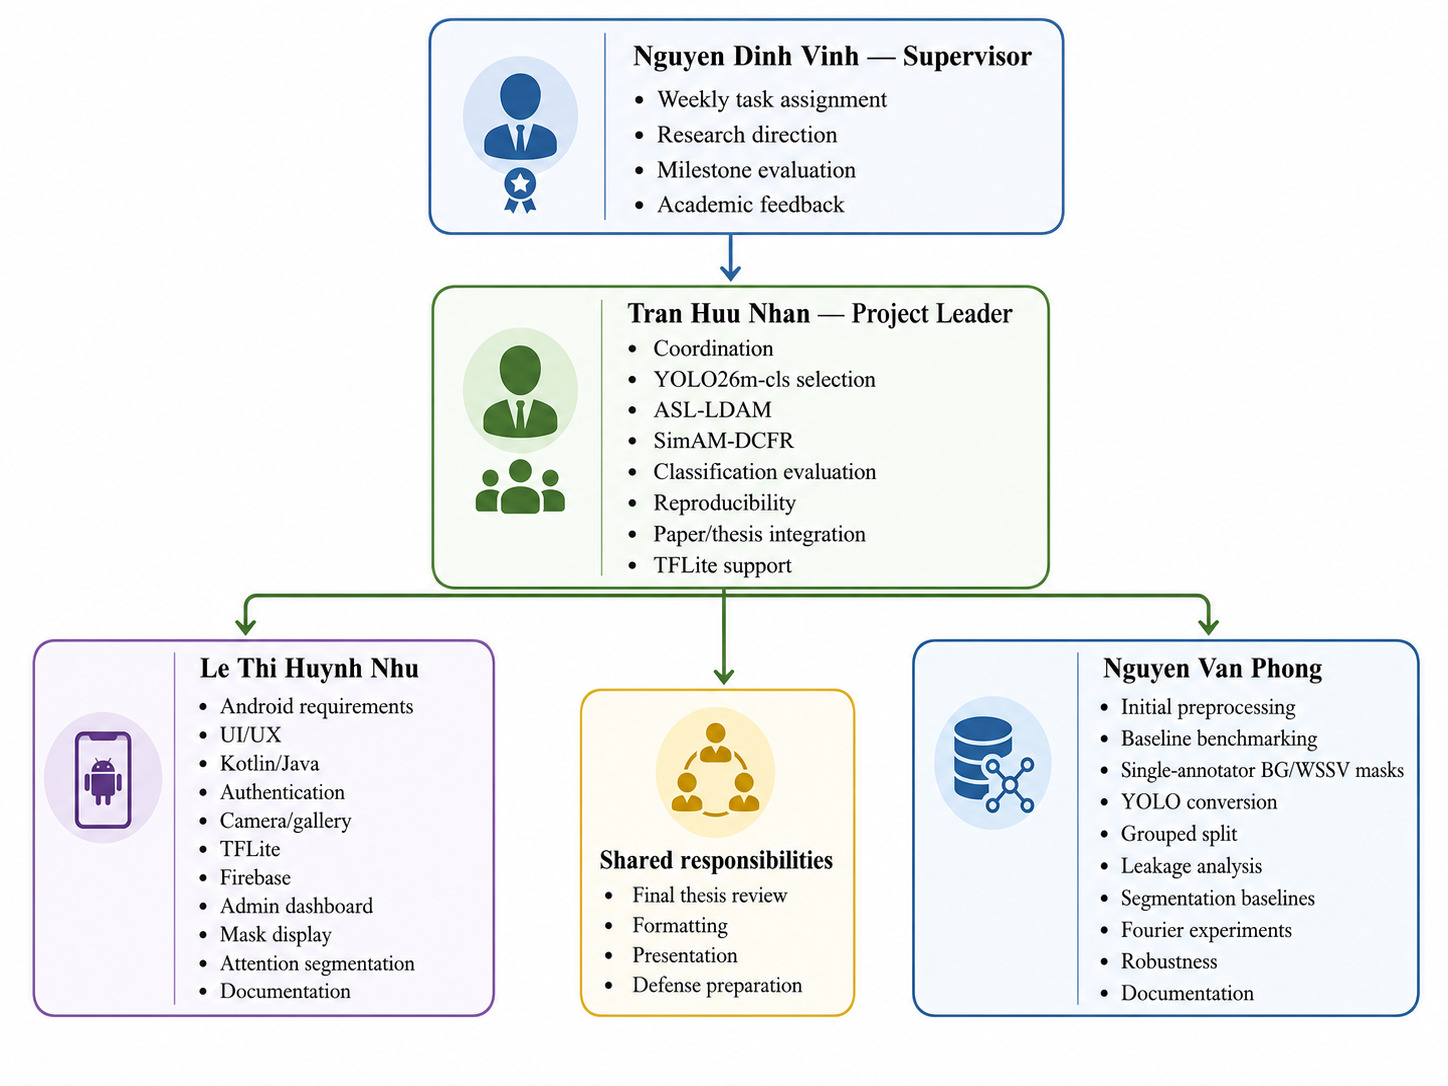
\includegraphics[width=0.94\textwidth,height=0.62\textheight,keepaspectratio]{assets/chapters_1_2/figure_2_1_team_structure.jpeg}
\caption{Team structure and research responsibilities.}
\end{figure}
The figure is positioned directly within the Team Structure and Roles subsection because it is the visual representation of the organizational arrangement. The shared-responsibility node indicates that all members participate in final thesis review, formatting, presentation, and defense preparation.\par
\begingroup
\CVioTableSetup
\begin{longtable}{|>{\centering\arraybackslash}p{3.54cm}|>{\centering\arraybackslash}p{10.43cm}|}
\caption{Roles and responsibilities}\\
\hline
\CVioPeachHeader\textbf{Role} & \textbf{Responsibility} \\ \hline
\endfirsthead
\caption[]{Roles and responsibilities (continued)}\\
\hline
\CVioPeachHeader\textbf{Role} & \textbf{Responsibility} \\ \hline
\endhead
\hline
\multicolumn{2}{r}{\footnotesize Continued on next page}\\
\endfoot
\hline
\endlastfoot
Supervisor & Assign weekly research tasks; review evidence, scope, protocols, and milestones; provide academic approval and feedback. \\ \hline
Project Leader & Coordinate schedule and dependencies; support members; lead classification research; integrate results, mobile model support, reproducibility artifacts, paper writing, and thesis delivery. \\ \hline
Mobile and Attention Lead & Develop the Android/Firebase application and conduct attention-based instance segmentation research and documentation. \\ \hline
Dataset and Fourier Lead & Lead initial dataset analysis, baseline benchmarking, single-annotator mask creation, grouped splitting, leakage analysis, Fourier experiments, robustness evaluation, and technical documentation. \\ \hline
All Members & Review final thesis content, verify figures and tables, prepare presentation material, and support defense preparation. \\ \hline
\end{longtable}
\endgroup
\subsubsection{Organizational Design Rationale}
The organizational structure is deliberately small and specialization-oriented. A single supervisor provides academic direction and milestone evaluation, while the project leader connects the classification, segmentation, mobile, and documentation workstreams. This structure avoids creating artificial software-company roles that do not match the project. The team does not have separate product-owner, Scrum-master, quality-assurance, or database-administrator positions. Instead, responsibility is assigned according to the research artifact that must be produced and reviewed.\par
The project leader is positioned as the integration point because classification research, TensorFlow Lite conversion, reproducibility packaging, paper writing, and final thesis assembly share common dependencies. This role includes tracking whether datasets, class orders, checkpoints, figures, and reported metrics remain consistent across experiments and documents. Coordination therefore extends beyond deadline reminders: it includes detecting incompatible assumptions between workstreams and ensuring that accepted results can be incorporated into one coherent final project.\par
\subsubsection{Role Evolution Across Project Phases}
Role allocation changed when the research scope expanded. During the initial classification phase, Tran Huu Nhan identified the source dataset and Nguyen Van Phong led the first dataset inspection, preprocessing, and baseline-model benchmarking. After the first review and the formal addition of instance segmentation around Session 3, the work was separated more sharply. Nhan concentrated on YOLO26m-cls selection, ASL-LDAM, SimAM-DCFR, classification robustness, XAI, external classification experiments, and integration. Nhu combined Android/Firebase development with attention-based segmentation research. Phong took ownership of mask semantics, single-annotator labeling, grouped splitting, leakage analysis, segmentation baselines, and Fourier-domain experiments.\par
This transition allowed the team to preserve continuity in the classification track while adding a substantial localization track without abandoning the mobile application. It also created explicit integration points. Classification outputs and mobile class order had to remain synchronized; segmentation labels and mask displays had to use consistent BG/WSSV meanings; and both research tracks had to contribute traceable results to the same thesis. The team structure therefore reflects both specialization and controlled integration rather than isolated individual work.\par
\subsubsection{Accountability, Review, and Shared Work}
Primary ownership does not remove review responsibilities. The member marked as the operational owner must prepare the artifact, configuration, or result, while the project leader and supervisor verify whether the output can support the intended claim. For example, a completed experiment must identify the dataset split, seed, preprocessing, model configuration, checkpoint-selection rule, metric, and saved result. A completed annotation task must identify class semantics, format, negative-image handling, and the known limitation that no independent expert mask review was performed.\par
Shared responsibilities are concentrated near major delivery points. All members review the final thesis, inspect figure and table consistency, prepare the presentation, rehearse the demonstration path, and support defense preparation. This shared review is necessary because the thesis integrates multiple technical tracks and because a local inconsistency can affect the interpretation of the whole project. Collective review does not replace ownership; it functions as a final cross-workstream verification layer.\par
\subsection{Communication Plan}
Project communication is organized around one formal weekly Google Meet and continuous Zalo communication. The supervisor normally assigns tasks during the weekly meeting. The project leader then monitors deadlines, coordinates dependencies, and supports members. Most assigned work is expected before the next weekly review so that results can be discussed and used to define the next task cycle. Blockers are reported immediately through Zalo and escalated to Google Meet when direct technical discussion is required.\par
\begingroup
\CVioTableSetup
\begin{longtable}{|>{\centering\arraybackslash}p{3.19cm}|>{\centering\arraybackslash}p{6.37cm}|>{\centering\arraybackslash}p{1.86cm}|>{\centering\arraybackslash}p{2.56cm}|}
\caption{Project communication plan}\\
\hline
\CVioPeachHeader\textbf{Communication item} & \textbf{Participants and purpose} & \textbf{Frequency} & \textbf{Tool / method} \\ \hline
\endfirsthead
\caption[]{Project communication plan (continued)}\\
\hline
\CVioPeachHeader\textbf{Communication item} & \textbf{Participants and purpose} & \textbf{Frequency} & \textbf{Tool / method} \\ \hline
\endhead
\hline
\multicolumn{4}{r}{\footnotesize Continued on next page}\\
\endfoot
\hline
\endlastfoot
Weekly progress and task meeting & Supervisor and all members. Review completed work, inspect evidence, discuss blockers, assign next tasks and assign next tasks & Weekly & Google Meet \\ \hline
Technical blocker discussion & Relevant members; project leader; supervisor when required. Resolve data, model, mobile, Firebase, conversion, or integration blockers & As needed & Zalo and Google Meet \\ \hline
Experiment review & AI members and project leader. Check split policy, settings, checkpoints, metrics, plots, and interpretation & Weekly / as needed & Google Meet, Kaggle, Google Drive \\ \hline
Document review & Authors, reviewers, project leader, supervisor. Review thesis structure, wording, tables, figures, citations, and accepted revisions & Before milestones & Google Docs and Google Meet \\ \hline
Quick coordination & All members. Share status, short files, reminders, and urgent questions & Continuous & Zalo \\ \hline
Repository synchronization & Technical members. Synchronize source code, notebooks, configurations, and documentation & Before review and release & Git and GitHub \\ \hline
\end{longtable}
\endgroup
The communication plan does not claim formal Scrum events. Weekly meetings combine evidence review, feedback, replanning, and task assignment. Zalo is a supporting communication channel, while Google Drive, Google Docs, GitHub, and Kaggle contain the principal research and document artifacts.\par
\subsubsection{Communication Cadence and Decision Flow}
The weekly Google Meet is the formal decision point of the project. Each meeting begins with the results and unresolved issues from the previous task cycle. Members report what was attempted, which artifacts were produced, whether the expected acceptance condition was met, and which technical or scheduling constraints remain. The supervisor then provides direction and assigns the next work, while the project leader records ownership, dependencies, and the expected deadline. In most weeks, the deadline is placed before the following meeting so that the next discussion is based on current evidence rather than unverified progress statements.\par
Communication is therefore result-centered. A statement that training was completed is insufficient unless the relevant logs, checkpoint, metrics, and configuration are available. Similarly, a claim that a dataset is ready must be supported by counts, manifests, class mapping, mask format, or split checks. This evidence-centered cadence reduces ambiguity and makes weekly decisions easier to trace to the WBS and Meeting Minutes.\par
\subsubsection{Blocker Escalation and Technical Resolution}
Zalo is used for immediate coordination because technical blockers do not always occur near the scheduled weekly meeting. A blocker may concern dataset access, an invalid label, a failed training run, incompatible model operators, unexpected metric changes, Firebase behavior, document formatting, or dependency delays. The responsible member reports the issue as soon as it is identified, and the project leader determines whether it can be resolved directly or requires supervisor discussion.\par
Escalation is proportionate to impact. A local implementation defect can be corrected without changing the project plan if it does not alter the dataset, metric, comparison protocol, or deadline. A blocker that changes a model configuration, invalidates a result, affects another member, or threatens a milestone is raised in Google Meet and recorded. This distinction prevents both extremes: silently changing important experimental conditions and over-formalizing minor technical corrections.\par
\subsubsection{Communication Records and Artifact Traceability}
Different communication tools serve different purposes. Google Meet supports formal review and task assignment. Zalo supports rapid coordination and short exchanges. Google Docs and Google Drive support collaborative writing, figures, reports, and meeting records. GitHub stores source code, configurations, and reproducibility documentation. Kaggle stores datasets, notebooks, training outputs, checkpoints, and result logs generated on the experiment platform. The project does not treat chat history as the final source of technical evidence.\par
A decision is considered traceable when the reason for the decision, the affected artifact, and the resulting update can be located. For example, the expansion to instance segmentation is reflected in Meeting Minutes, ownership assignments, WBS tasks, new dataset preparation, segmentation experiments, mobile mask-display requirements, and thesis scope. This multi-artifact consistency is important because management decisions and scientific claims must describe the same project state.\par
\section{Project Management Approach}
The project uses CRISP-DM as the named process model because it is an established data-mining and machine-learning lifecycle that matches the project emphasis on problem definition, data understanding, data preparation, modeling, evaluation, and deployment. The project does not rename CRISP-DM or claim a new official process model. Instead, the team applies the original phases iteratively and uses a weekly supervisor-controlled execution cycle to manage research tasks and evidence.\par
Figure 2.2 maps the original six CRISP-DM phases to the project. Dataset and experimental evidence are placed at the center because data quality, split validity, labeling, and traceable experiment outputs influence every phase.\par
\begin{figure}[tbp]
\centering
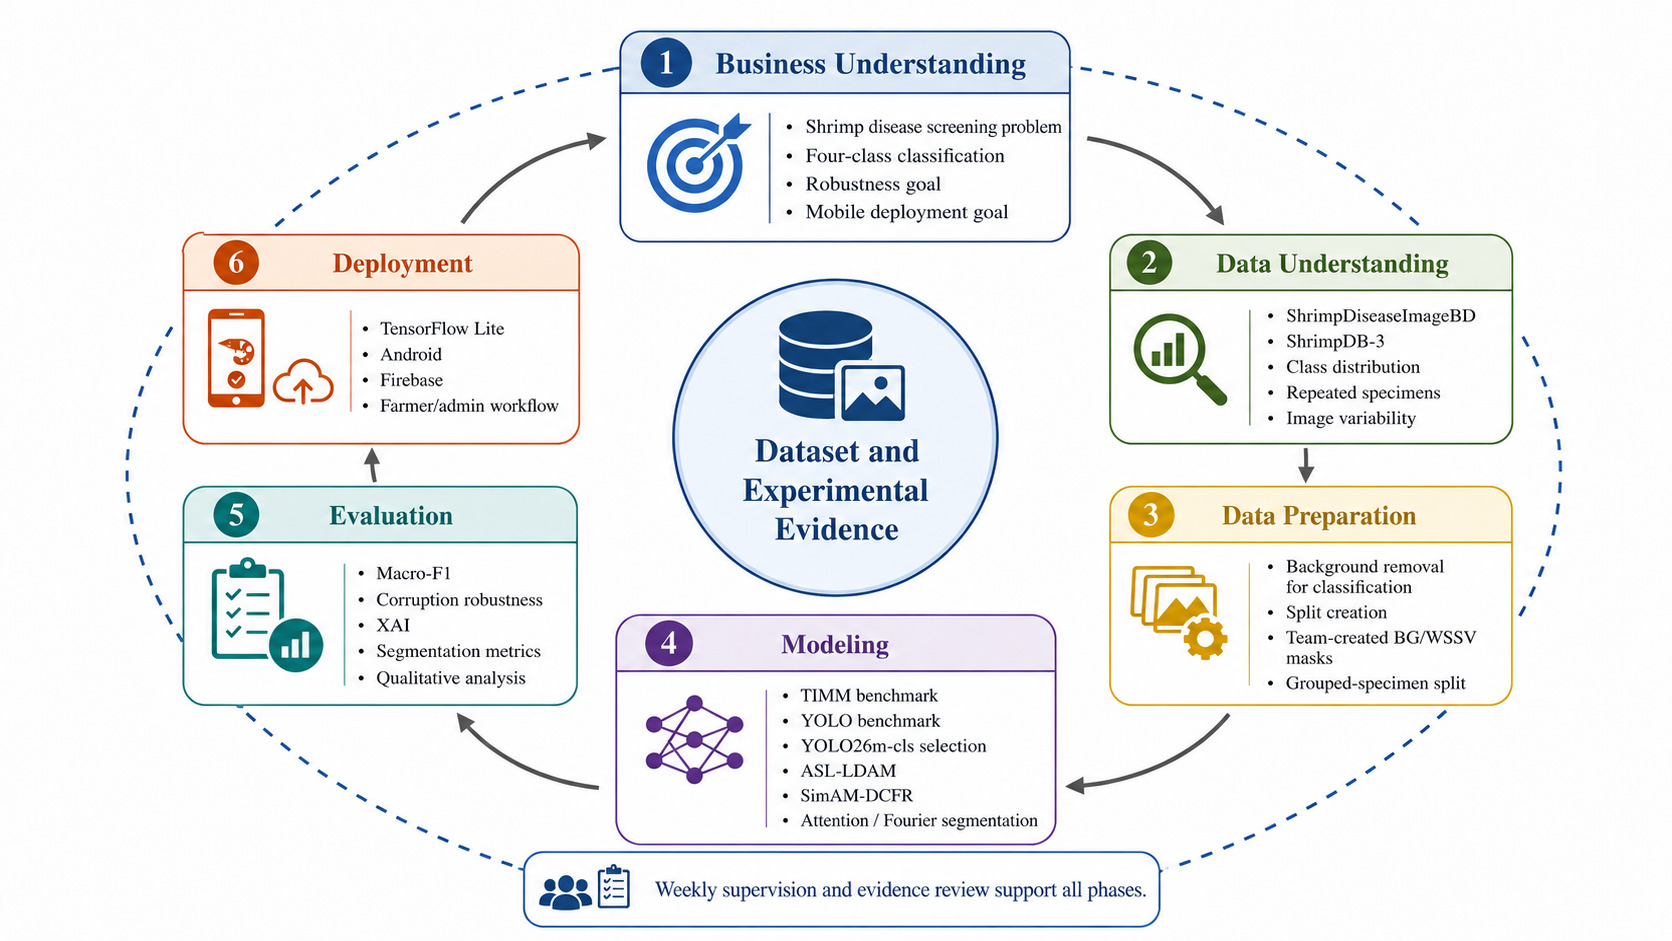
\includegraphics[width=0.94\textwidth,height=0.62\textheight,keepaspectratio]{assets/chapters_1_2/figure_2_2_crisp_dm.jpeg}
\caption{CRISP-DM applied to the project.}
\end{figure}
The circular structure emphasizes iteration. Evaluation can send the project back to data preparation or modeling, and deployment findings can trigger further model or preprocessing revisions. Weekly supervision and evidence review operate across all phases rather than forming a seventh CRISP-DM phase.\par
\begingroup
\CVioTableSetup
\begin{longtable}{|>{\centering\arraybackslash}p{3.54cm}|>{\centering\arraybackslash}p{10.43cm}|}
\caption{Application of CRISP-DM phases to the project}\\
\hline
\CVioPeachHeader\textbf{CRISP-DM phase} & \textbf{project application} \\ \hline
\endfirsthead
\caption[]{Application of CRISP-DM phases to the project (continued)}\\
\hline
\CVioPeachHeader\textbf{CRISP-DM phase} & \textbf{project application} \\ \hline
\endhead
\hline
\multicolumn{2}{r}{\footnotesize Continued on next page}\\
\endfoot
\hline
\endlastfoot
Business Understanding & Define preliminary shrimp disease screening, four-class classification, robustness, model efficiency, and mobile deployment goals. \\ \hline
Data Understanding & Inspect ShrimpDiseaseImageBD and ShrimpDB, class distributions, image variability, duplicates, and repeated specimens. \\ \hline
Data Preparation & Perform classification-specific background removal, fixed splitting, mask annotation, class mapping, and grouped-specimen splitting. \\ \hline
Modeling & Benchmark TIMM and YOLO models; develop ASL-LDAM, SimAM-DCFR, attention segmentation, and Fourier-domain variants. \\ \hline
Evaluation & Use Macro-F1, Kappa, robustness testing, XAI, segmentation metrics, qualitative analysis, and leakage comparison. \\ \hline
Deployment & Deploy classifier + segmenter as a conditional Android TFLite cascade; integrate Firebase and user/admin workflows. \\ \hline
\end{longtable}
\endgroup
The formal CRISP-DM lifecycle is executed through the weekly research cycle shown in Figure 2.3. The supervisor assigns a task, members research and implement the method, experiments generate evidence, evaluation determines the result, and the weekly review decides whether to revise, continue, or replace the task.\par
\begin{figure}[tbp]
\centering
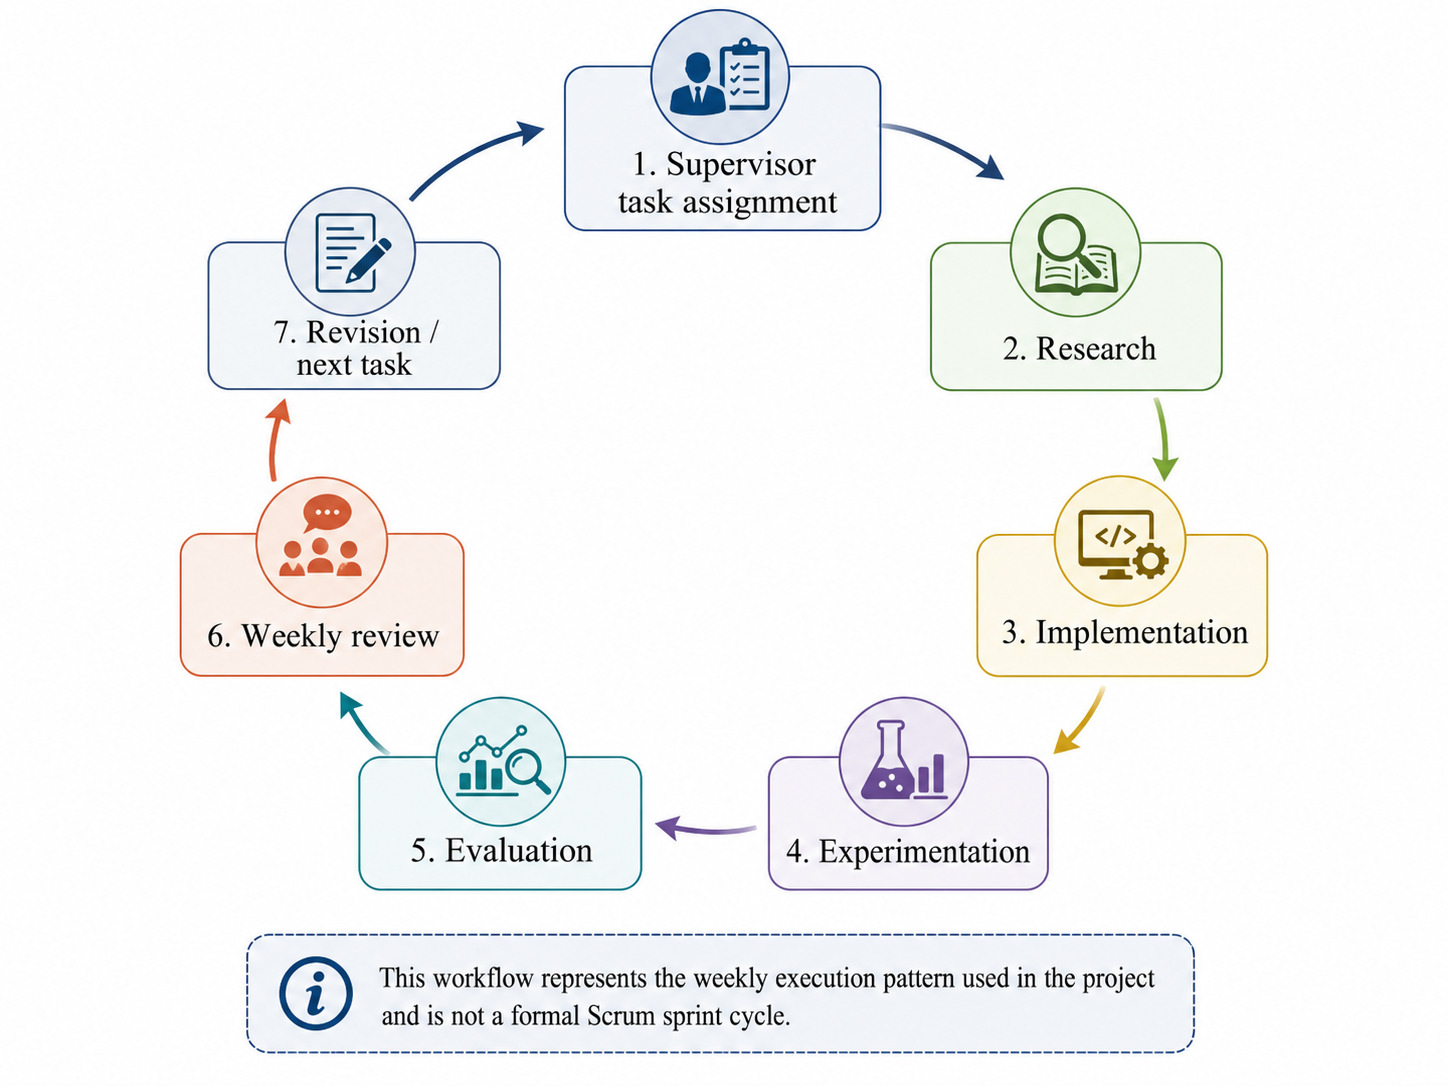
\includegraphics[width=0.94\textwidth,height=0.62\textheight,keepaspectratio]{assets/chapters_1_2/figure_2_3_weekly_cycle.jpeg}
\caption{Weekly research execution cycle.}
\end{figure}
This workflow is not a formal Scrum sprint because the project does not conduct daily Scrum events, formal sprint retrospectives, or a software-testing-driven increment for every week. It is a research execution pattern in which experimental evidence, implementation feasibility, and supervisor feedback determine the next action.\par
CRISP-DM was selected because it provides a recognized lifecycle for projects in which data characteristics, preparation choices, model behavior, evaluation findings, and deployment constraints repeatedly influence one another. The framework is more suitable than a formal Scrum description for the project because weekly work is driven by research questions and experimental outcomes rather than by a fixed software increment and a complete test suite. The six CRISP-DM phase names are retained without inventing a new methodology name.\par
Business Understanding establishes the initial four-class classification, robustness, lightweight deployment, intended users, and non-clinical boundary. Data Understanding investigates source datasets, class distribution, image variability, repeated specimens, and annotation feasibility. Data Preparation is task-specific: classification uses background removal and fixed image-level partitions, whereas segmentation requires team-created disease-region masks, Healthy empty-label negatives, and later a grouped-specimen split. These differences prevent the project from applying one preprocessing assumption indiscriminately to both tasks.\par
Modeling includes controlled screening of TIMM and official Ultralytics classification models, selection of YOLO26m-cls under the performance and approximate parameter constraint, implementation of ASL-LDAM and SimAM-DCFR, and the segmentation attention and Fourier studies. Evaluation checks clean performance, corruption behavior, classwise outcomes, qualitative XAI, mask metrics, leakage effects, and failure cases. Deployment converts selected outputs into Android, TensorFlow Lite, Firebase, farmer, and administrator workflows. Findings in any later phase may require revision of an earlier phase.\par
The weekly execution cycle operationalizes CRISP-DM without changing its official phases. A weekly task may begin in one phase and return to another after evaluation. For example, an unexpected segmentation result may trigger a label audit, a grouped-split revision, or a new modeling hypothesis. A mobile conversion failure may trigger architecture or preprocessing changes. This iterative interpretation makes the management approach consistent with the actual uncertainty of AI research.\par
\subsection{WBS}
The Work Breakdown Structure organizes the project into planning, dataset preparation, model development, mobile integration, documentation, and closure tasks. One man-day equals eight hours, and the estimates include both active work and scheduled experiment execution.\par
\rev{
Classification uses the fixed seed-42 nominal 70/15/15 split. Segmentation retains Healthy images as empty-label negatives and uses a nominal 80/10/10 specimen-grouped split when filenames expose compatible specimen identities. The 303 unmatched-name additions lack recoverable specimen IDs and therefore use image-level stratified splitting; the expanded inventory is not claimed to be fully specimen-leakage-free.
}
\rev{
Modeling screens TIMM and official Ultralytics classifiers. YOLO26m-cls is retained under a deployment-oriented preference of approximately 15M parameters or fewer; larger candidates remain diagnostic references rather than eligible final mobile candidates. Subsequent work covers ASL-LDAM, SimAM-DCFR, and attention/Fourier segmentation. Deployment uses a conditional Android TFLite classifier-segmenter cascade.
}
\begingroup
\CVioTableSetup
\scriptsize
\begin{longtable}{|>{\centering\arraybackslash}p{1.07cm}|>{\centering\arraybackslash}p{8.22cm}|>{\centering\arraybackslash}p{2.30cm}|>{\centering\arraybackslash}p{2.12cm}|}
\caption{Detailed Work Breakdown Structure and estimated effort}\\
\hline
\CVioPeachHeader\textbf{\#} & \textbf{WBS Item} & \textbf{Complexity} & \textbf{Est. effort (man-days)} \\ \hline
\endfirsthead
\caption[]{Detailed Work Breakdown Structure and estimated effort (continued)}\\
\hline
\CVioPeachHeader\textbf{\#} & \textbf{WBS Item} & \textbf{Complexity} & \textbf{Est. effort (man-days)} \\ \hline
\endhead
\hline
\multicolumn{4}{r}{\footnotesize Continued on next page}\\
\endfoot
\hline
\endlastfoot
\textbf{1} & \textbf{Project planning and governance} & \textbf{} & \textbf{} \\ \hline
1.1 & Confirm initial project scope and intended users & Simple & 2 \\ \hline
1.2 & Establish weekly supervisor review cycle & Simple & 2 \\ \hline
1.3 & Create communication and escalation channels & Simple & 2 \\ \hline
1.4 & Create GitHub repository and branch structure & Medium & 3 \\ \hline
1.5 & Create Google Drive and Google Docs workspace & Simple & 2 \\ \hline
1.6 & Prepare meeting-minute templates and tracking rules & Simple & 2 \\ \hline
1.7 & Maintain milestone and deadline tracking & Medium & 6 \\ \hline
1.8 & Review project scope after Session 3 & Medium & 2 \\ \hline
1.9 & Integrate instance segmentation into the official scope & Medium & 3 \\ \hline
\textbf{2} & \textbf{Classification dataset preparation} & \textbf{} & \textbf{} \\ \hline
2.1 & Locate and verify ShrimpDiseaseImageBD source & Simple & 2 \\ \hline
2.2 & Inspect class folders and image counts & Medium & 3 \\ \hline
2.3 & Check duplicates and repeated specimens & Complex & 5 \\ \hline
2.4 & Implement background-removal preprocessing & Complex & 6 \\ \hline
2.5 & Audit preprocessing outputs by class & Medium & 3 \\ \hline
2.6 & Create fixed seed-42 train/validation/test split & Medium & 4 \\ \hline
2.7 & Export split manifests and class statistics & Simple & 2 \\ \hline
2.8 & Prepare EXT-3-Original class mapping & Medium & 3 \\ \hline
2.9 & Prepare SDI-4 + EXT-3-Original partition-wise merge & Complex & 5 \\ \hline
2.10 & Verify cross-partition source integrity & Complex & 4 \\ \hline
\textbf{3} & \textbf{Classification baseline benchmarking} & \textbf{} & \textbf{} \\ \hline
3.1 & Define lightweight parameter budget and metrics & Medium & 3 \\ \hline
3.2 & Benchmark ConvNeXt and representative TIMM models & Complex & 8 \\ \hline
3.3 & Benchmark YOLOv8 classification variants & Complex & 5 \\ \hline
3.4 & Benchmark YOLO11 classification variants & Complex & 5 \\ \hline
3.5 & Benchmark YOLO26 classification variants & Complex & 5 \\ \hline
3.6 & Collect parameter count, size, latency, FPS, and metrics & Complex & 5 \\ \hline
3.7 & Compare TIMM and YOLO efficiency-performance trade-offs & Complex & 4 \\ \hline
3.8 & Select YOLO26m-cls as the improvement backbone & Medium & 2 \\ \hline
\textbf{4} & \textbf{Proposed classification method} & \textbf{} & \textbf{} \\ \hline
4.1 & Review imbalance-aware loss literature & Complex & 4 \\ \hline
4.2 & Design ASL-LDAM objective & Complex & 6 \\ \hline
4.3 & Implement ASL-LDAM in the training pipeline & Complex & 7 \\ \hline
4.4 & Review SimAM and feature-recalibration literature & Complex & 4 \\ \hline
4.5 & Implement SimAM gated residual integration & Complex & 6 \\ \hline
4.6 & Design and implement DCFR texture recalibration & Complex & 8 \\ \hline
4.7 & Integrate SimAM-DCFR with YOLO26m-cls & Complex & 7 \\ \hline
4.8 & Run component-level ablation study & Complex & 8 \\ \hline
4.9 & Select and freeze the final proposed checkpoint & Medium & 3 \\ \hline
4.10 & Evaluate clean test performance & Medium & 3 \\ \hline
4.11 & Evaluate corruption robustness & Complex & 7 \\ \hline
4.12 & Generate Grad-CAM-based XAI evidence & Complex & 5 \\ \hline
4.13 & Run EXT-3-Original classification experiment & Complex & 5 \\ \hline
4.14 & Run SDI-4 + EXT-3-Original classification experiment & Complex & 5 \\ \hline
4.15 & Package classification reproducibility artifacts & Complex & 6 \\ \hline
\textbf{5} & \textbf{Instance-segmentation dataset preparation} & \textbf{} & \textbf{} \\ \hline
5.1 & Define BG/WSSV disease-region mask semantics & Complex & 4 \\ \hline
5.2 & Create single-annotator labeling protocol & Medium & 3 \\ \hline
5.3 & Label BG disease regions & Complex & 12 \\ \hline
5.4 & Label WSSV disease regions & Complex & 14 \\ \hline
5.5 & Label co-infection images with both mask classes & Complex & 8 \\ \hline
\rev{5.6} & \rev{Retain Healthy images as empty-label negatives} & \rev{Simple} & \rev{2} \\ \hline
5.7 & Convert masks to YOLO segmentation format & Complex & 5 \\ \hline
5.8 & Generate annotation statistics and examples & Medium & 3 \\ \hline
5.9 & Define specimen identifiers from filenames & Complex & 4 \\ \hline
\rev{5.10} & \rev{Create grouped-specimen split} & \rev{Complex} & \rev{6} \\ \hline
5.11 & Audit specimen overlap and leakage & Complex & 5 \\ \hline
5.12 & Prepare ShrimpDB segmentation annotations & Complex & 8 \\ \hline
\textbf{6} & \textbf{Instance-segmentation modeling} & \textbf{} & \textbf{} \\ \hline
6.1 & Benchmark YOLOv8-seg variants & Complex & 6 \\ \hline
6.2 & Benchmark YOLO11-seg variants & Complex & 6 \\ \hline
6.3 & Benchmark YOLO26-seg variants & Complex & 6 \\ \hline
\rev{6.4} & \rev{Select grouped-split segmentation baseline} & \rev{Medium} & \rev{3} \\ \hline
6.5 & Review lightweight attention mechanisms & Complex & 4 \\ \hline
6.6 & Implement attention modules in segmentation backbone & Complex & 8 \\ \hline
6.7 & Run attention segmentation experiments & Complex & 9 \\ \hline
6.8 & Document attention ablation results & Medium & 4 \\ \hline
\rev{6.9} & \rev{Review Fourier-domain augmentation methods} & \rev{Complex} & \rev{5} \\ \hline
\rev{6.10} & \rev{Implement Fourier transformation variants} & \rev{Complex} & \rev{8} \\ \hline
\rev{6.11} & \rev{Run Fourier segmentation experiments} & \rev{Complex} & \rev{9} \\ \hline
6.12 & Evaluate segmentation under task-specific corruptions & Complex & 7 \\ \hline
6.13 & Analyze qualitative predictions and failure cases & Complex & 5 \\ \hline
6.14 & Package segmentation reproducibility artifacts & Complex & 5 \\ \hline
\textbf{7} & \textbf{Mobile application and Firebase} & \textbf{} & \textbf{} \\ \hline
7.1 & Analyze farmer and administrator requirements & Medium & 4 \\ \hline
7.2 & Design Android UI/UX flows & Complex & 7 \\ \hline
7.3 & Implement registration and authentication & Complex & 7 \\ \hline
7.4 & Implement camera and gallery image input & Complex & 6 \\ \hline
\rev{7.5} & \rev{Package final two-model TFLite bundle} & \rev{Complex} & \rev{7} \\ \hline
7.6 & Implement conditional Android CPU inference & Complex & 8 \\ \hline
7.7 & Implement classification result display & Medium & 5 \\ \hline
7.8 & Implement segmentation mask display & Complex & 7 \\ \hline
7.9 & Implement history, export, and delete operations & Complex & 7 \\ \hline
7.10 & Integrate Firebase data services & Complex & 8 \\ \hline
7.11 & Implement administrator dashboard & Complex & 8 \\ \hline
\rev{7.12} & \rev{Capture three-device runtime evidence} & \rev{Medium} & \rev{4} \\ \hline
\textbf{8} & \textbf{Documentation, publication, and closure} & \textbf{} & \textbf{} \\ \hline
8.1 & Write classification paper draft & Complex & 10 \\ \hline
8.2 & Write segmentation technical sections & Complex & 8 \\ \hline
8.3 & Write project introduction and management plan & Complex & 7 \\ \hline
8.4 & Integrate methodology and experimental results & Complex & 10 \\ \hline
8.5 & Audit terminology, figures, and tables & Complex & 6 \\ \hline
8.6 & Verify metric and checkpoint traceability & Complex & 6 \\ \hline
8.7 & Prepare final GitHub documentation & Complex & 5 \\ \hline
8.8 & Prepare presentation and defense materials & Complex & 6 \\ \hline
8.9 & Conduct final thesis review and formatting & Complex & 8 \\ \hline
\rev{8.10} & \rev{Submit initial defense DOCX package} & \rev{Simple} & \rev{2} \\ \hline
\textbf{} & \textbf{Total Estimated Effort (man-days)} & \textbf{} & \textbf{487} \\ \hline
\end{longtable}
\endgroup
Table 2.5 lists 90 executable tasks with a total estimated effort of 487 man-days. These values are planning estimates used to control workload, dependencies, and completion milestones.\par
\begin{figure}[tbp]
\centering
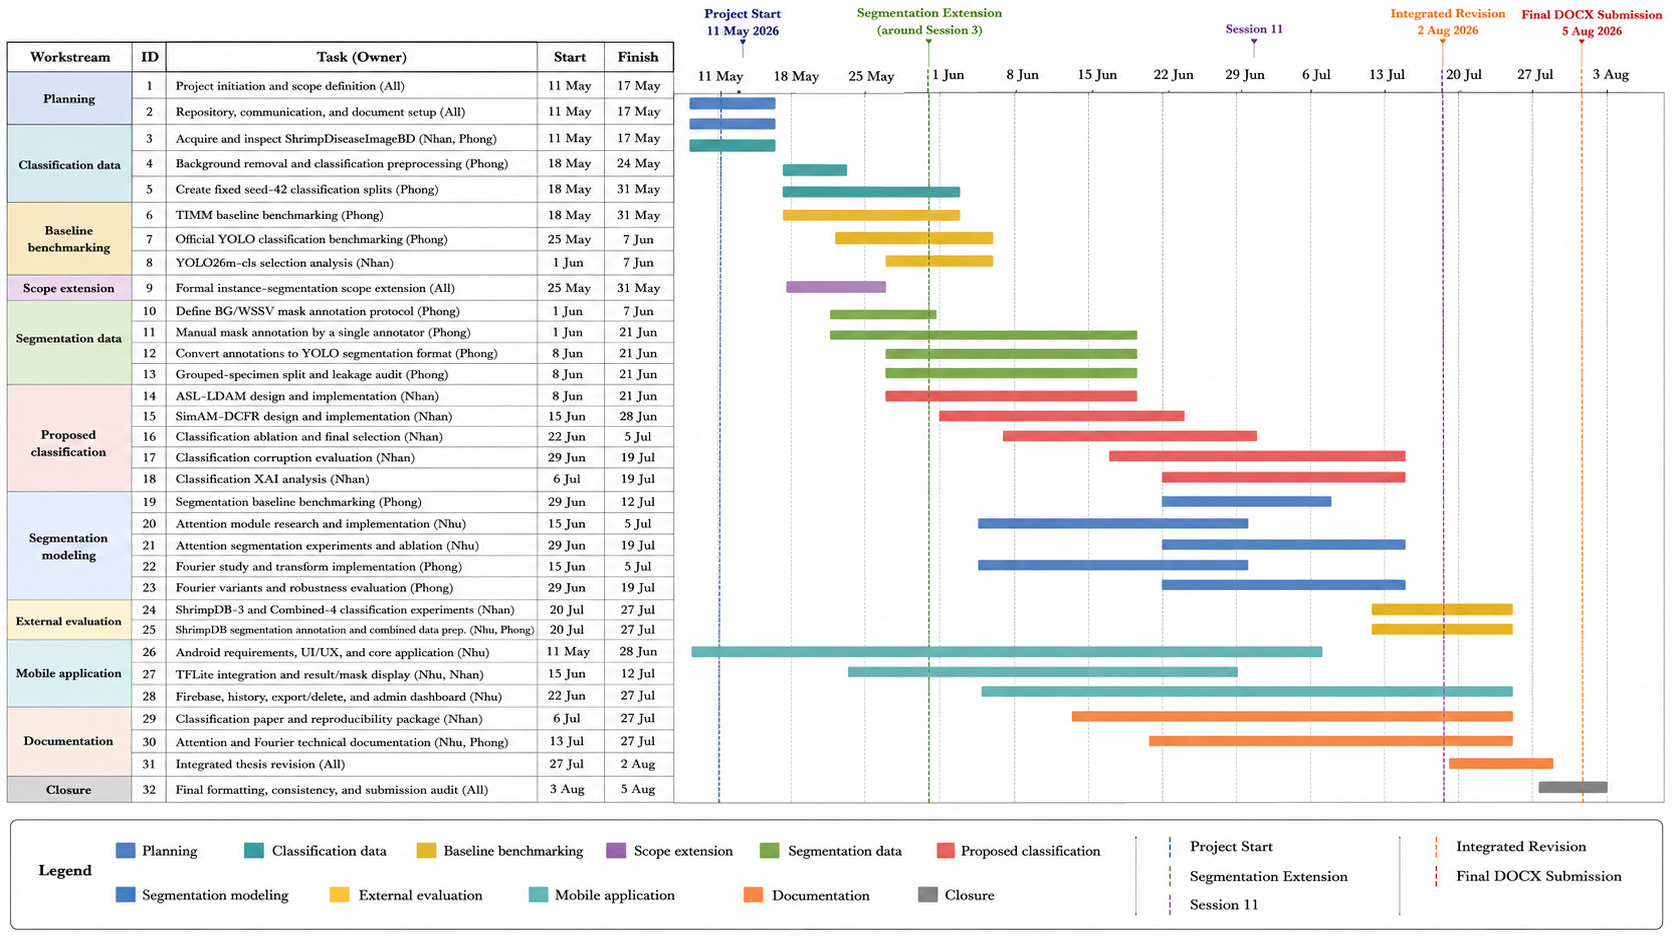
\includegraphics[width=0.98\textwidth,height=0.70\textheight,keepaspectratio]{assets/chapters_1_2/figure_2_4_gantt.jpeg}
\caption{Project Gantt chart.}
\end{figure}
\rev{
Figure 2.4 presents the baseline schedule from 11 May to the initial defense DOCX submission on 5 August 2026. Milestones mark project start, segmentation extension, Session 11, integrated revision, and the initial submission freeze.
}
\rev{
The Gantt chart is a planning model rather than an exact timestamp record. Dates are reconstructed from Meeting Minutes 1-11, milestones, dependencies, and the initial pre-defense submission on 5 August 2026. The later Council No. 03 revision cycle is tracked separately under change management. Weekly review compares planned and actual state, identifies unfinished dependencies, and adjusts the next task allocation.
}
\begingroup
\CVioTableSetup
\scriptsize
\begin{longtable}{|>{\centering\arraybackslash}p{3.98cm}|>{\centering\arraybackslash}p{2.30cm}|>{\centering\arraybackslash}p{2.30cm}|>{\centering\arraybackslash}p{2.30cm}|>{\centering\arraybackslash}p{2.30cm}|}
\caption{Responsibility assignments}\\
\hline
\CVioPeachHeader\textbf{Responsibility} & \textbf{Tran Huu Nhan} & \textbf{Le Thi Huynh Nhu} & \textbf{Nguyen Van Phong} & \textbf{Nguyen Dinh Vinh} \\ \hline
\endfirsthead
\caption[]{Responsibility assignments (continued)}\\
\hline
\CVioPeachHeader\textbf{Responsibility} & \textbf{Tran Huu Nhan} & \textbf{Le Thi Huynh Nhu} & \textbf{Nguyen Van Phong} & \textbf{Nguyen Dinh Vinh} \\ \hline
\endhead
\hline
\multicolumn{5}{r}{\footnotesize Continued on next page}\\
\endfoot
\hline
\endlastfoot
Project planning and weekly tracking & R & S & S & D \\ \hline
Initial dataset analysis and preprocessing & S & S & D & R \\ \hline
TIMM and YOLO baseline benchmarking & S & I & D & R \\ \hline
YOLO26m-cls selection and proposed classification & D & I & S & R \\ \hline
Classification robustness and XAI & D & I & S & R \\ \hline
BG/WSSV mask annotation and YOLO conversion & S & I & D & R \\ \hline
Grouped split and leakage analysis & S & I & D & R \\ \hline
Attention segmentation research & S & D & R & R \\ \hline
Fourier segmentation research & S & R & D & R \\ \hline
Android, Firebase, and administrator dashboard & S & D & I & R \\ \hline
Reproducibility packaging and GitHub documentation & D & S & S & R \\ \hline
Final thesis integration and formatting & D & D & D & R \\ \hline
Presentation and defense preparation & D & D & D & R \\ \hline
\end{longtable}
\endgroup
Responsibility codes are defined as D = Do, R = Review, S = Support, and I = Informed. The matrix identifies operational ownership without replacing the detailed role descriptions in Tables 2.1 and 2.2.\par
\subsubsection{WBS Design Principles}
The WBS decomposes the project by deliverable and research responsibility rather than by generic development activity. Parent work packages represent planning and governance, classification data, baseline benchmarking, proposed classification, segmentation data, segmentation modeling, mobile integration, and final documentation and closure. Child tasks are sufficiently specific to assign an owner and define an output, but they do not descend into trivial operations that would make the schedule unreadable.\par
Research tasks are separated when they have different acceptance conditions. Literature review, implementation, controlled training, ablation, robustness evaluation, external evaluation, qualitative interpretation, and reproducibility packaging are not treated as one combined task. This decomposition makes it possible to identify where a claim originated and whether the required supporting evidence was actually completed.\par
\subsubsection{Effort Estimation Assumptions}
One man-day is defined as eight hours for estimation. Because the project is a capstone rather than contracted employment, the estimate is used as a workload and scheduling measure, not as payroll accounting. Work may occur on any day of the week, and the team is evaluated by completion of assigned tasks rather than by a fixed office calendar. The schedule therefore records estimated effort and deadlines without claiming a conventional five-day employment pattern.\par
The user-approved estimation policy includes monitored GPU execution within the task effort because a long experiment occupies an assigned task, requires configuration, observation, checkpoint handling, failure recovery, and result extraction. This does not imply that unattended compute is equivalent to continuous human labor. It indicates that experiment duration consumes project time and affects dependencies. The 487 man-day total is consequently a planning aggregate that combines active work and allocated experiment completion time.\par
\subsubsection{Dependency and Parallel-Execution Logic}
Dependencies protect scientific validity. Classification model comparison depends on a fixed dataset split and consistent metrics. Proposed-method experiments depend on the selected YOLO26m-cls baseline. Corruption and XAI analysis depend on a frozen checkpoint. Segmentation benchmarking depends on mask conversion and the grouped split. Attention and Fourier comparisons depend on the same baseline protocol. Mobile inference depends on a validated model conversion and stable class order. Documentation depends on results that have passed consistency checks.\par
Parallelism is used when dependencies permit it. Android UI and application infrastructure begin early while model research continues. Attention and Fourier segmentation are developed by different members after the common dataset preparation becomes available. Classification paper writing begins before all final thesis sections are integrated, while reproducibility packaging overlaps late experiments. This controlled parallelism shortens the project calendar without treating dependent outputs as interchangeable.\par
\subsubsection{Interpretation of the Main Work Packages}
The planning and governance package establishes the initial scope, collaboration environment, weekly review cycle, and scope-extension record. The classification-data package verifies the source dataset, performs ShrimpXNet-inspired background removal for the classification track, creates the seed-42 partitions, and prepares source-wise external datasets. The baseline package compares representative TIMM and official YOLO models so that YOLO26m-cls is selected from measured evidence rather than preference.\par
\rev{
The proposed-classification package covers ASL-LDAM, SimAM-DCFR, component evidence, clean and corruption evaluation, XAI, external retraining, and reproducibility packaging. Segmentation packages cover mask semantics, Healthy empty-label handling, grouped splitting and leakage, baselines, attention, Fourier variants, robustness, and failure analysis. Mobile work demonstrates practical integration. The final package controls papers, thesis assembly, GitHub
}
\subsubsection{Schedule Monitoring and Re-planning}
Schedule control prioritizes research validity over superficial completion. An experiment is not marked complete merely to preserve a date if the configuration is inconsistent or the evidence is missing. Conversely, non-critical polishing can be reduced when it threatens a required dataset, experiment, integration, or submission milestone. The WBS, Gantt chart, responsibility matrix, and Meeting Minutes together provide complementary views of task scope, time, ownership, and decision history.\par
\subsection{Risk Management}
Risk management focuses on threats that can invalidate research conclusions, delay integration, or produce unsupported deployment claims. Each risk is associated with a preventive or corrective response.\par
\begingroup
\CVioTableSetup
\scriptsize
\begin{longtable}{|>{\centering\arraybackslash}p{0.88cm}|>{\centering\arraybackslash}p{4.24cm}|>{\centering\arraybackslash}p{3.00cm}|>{\centering\arraybackslash}p{5.49cm}|}
\caption{Project risks and response plans}\\
\hline
\CVioPeachHeader\textbf{\#} & \textbf{Risk description} & \textbf{Impact / likelihood} & \textbf{Response plan} \\ \hline
\endfirsthead
\caption[]{Project risks and response plans (continued)}\\
\hline
\CVioPeachHeader\textbf{\#} & \textbf{Risk description} & \textbf{Impact / likelihood} & \textbf{Response plan} \\ \hline
\endhead
\hline
\multicolumn{4}{r}{\footnotesize Continued on next page}\\
\endfoot
\hline
\endlastfoot
\rev{1} & \rev{Repeated-specimen leakage} & \rev{Impact: Critical; likelihood: Medium} & \rev{Group by specimen and audit overlap where filenames expose IDs; report unmatched-name additions separately because specimen identity is unavailable.} \\ \hline
\rev{2} & \rev{Single-annotator mask inconsistency} & \rev{Impact: High; likelihood: Medium} & \rev{Use one documented labeling policy for consistency; disclose the absence of independent expert review as a limitation.} \\ \hline
3 & Class imbalance and co-infection overlap & Impact: High; likelihood: High & Use Macro-F1, classwise analysis, ASL-LDAM, confusion matrices, and controlled ablations. \\ \hline
\rev{4} & \rev{Inconsistent baseline settings} & \rev{Impact: Critical; likelihood: Medium} & \rev{Fix dataset split, seed, preprocessing, checkpoint selection, metrics, class order, and evaluation scripts for direct comparisons.} \\ \hline
5 & Non-reproducible experimental result & Impact: High; likelihood: Medium & Archive configurations, environment metadata, checkpoints, logs, and exported result packages. \\ \hline
6 & GPU quota or long experiment time & Impact: Medium; likelihood: High & Prioritize critical experiments, checkpoint runs, use staged debugging, and adjust deadlines through weekly review. \\ \hline
7 & Mobile conversion or operator incompatibility & Impact: High; likelihood: Medium & Validate both TFLite artifacts, tensor shapes, class order, decoder, supported ops, and four-thread CPU path before deployment claims. \\ \hline
8 & Prototype latency too high & Impact: High; likelihood: High & Report branch-aware Android runtime; separate no-seg and segmentation-triggered paths; avoid pure-latency, strict ranking, and real-time claims. \\ \hline
9 & Firebase/network interruption & Impact: Medium; likelihood: Medium & Separate local inference from service failures; test authentication and persistence flows before demonstrations. \\ \hline
\rev{10} & \rev{Scope creep after review feedback} & \rev{Impact: High; likelihood: Medium} & \rev{Apply the change-management process; assess schedule and dependencies; update WBS and meeting minutes.} \\ \hline
\rev{11} & \rev{Overclaiming diagnosis or generalization} & \rev{Impact: Critical; likelihood: Medium} & \rev{Describe the system as preliminary screening; state dataset, annotation, corruption, mobile, and external-validation limitations explicitly.} \\ \hline
\rev{12} & \rev{Final document inconsistency} & \rev{Impact: High; likelihood: Medium} & \rev{Review before 5 August, then complete the Council-mandated cross-document audit and revised submission before 12:00 on 15 August 2026.} \\ \hline
\end{longtable}
\endgroup
The highest-priority risks are those that affect scientific validity: leakage, inconsistent settings, non-reproducible evidence, and overclaiming. Schedule and application risks remain important, but they\par
\subsubsection{Risk Identification and Prioritization}
Risk identification is performed from the perspective of research validity, delivery feasibility, and claim defensibility. A risk is considered critical when it can invalidate the comparison, create leakage, disconnect a reported metric from its checkpoint, or cause the thesis to make a claim unsupported by the available evidence. Operational inconvenience alone is not automatically critical unless it threatens a milestone or prevents completion of a required workstream.\par
Impact and possibility are assessed qualitatively because the project does not have sufficient historical data for calibrated probabilities. The classifications are used to focus attention, assign preventive controls, and determine escalation. High-impact risks are reviewed during weekly meetings, while immediate failures are reported through Zalo. The risk table records the agreed response rather than pretending that all uncertainty can be eliminated.\par
\subsubsection{Scientific-Validity Risks}
Repeated-specimen leakage can inflate segmentation performance when related shrimp views cross partitions. Grouped splitting and overlap audits control this for filename-compatible records. The 303 unmatched-name additions lack specimen IDs and use image-level splitting, so the expanded inventory is not claimed to be fully specimen-leakage-free.\par
Single-annotator masks improve internal labeling consistency but create uncertainty about clinical correctness and boundary subjectivity. The project addresses this by documenting mask semantics, using one protocol, treating Healthy images as empty-label negatives, and disclosing the absence of independent expert review. The limitation is not hidden by the use of precise polygon format or model metrics. Similar caution applies to XAI, which provides qualitative model-attention evidence but not causal or veterinary proof.\par
Inconsistent experimental settings are controlled because they can invalidate baseline comparisons more directly than a small metric difference. Dataset version, split, seed, preprocessing, augmentation, optimizer, checkpoint selection, class order, and evaluation code must be fixed or explicitly identified when comparing methods. The final classification result of 91.01\% Macro-F1 is required to be reported consistently in the final document according to the accepted project consolidation, and related tables, figures, and conclusions must use the same interpretation.\par
\subsubsection{Resource, Integration, and Schedule Risks}
Kaggle GPU availability, long training time, failed runs, and storage limits can delay research. The response is to debug with staged experiments, preserve checkpoints, prioritize the experiments necessary for the declared contributions, and revise deadlines through the weekly process. The project avoids presenting every attempted run as equally important; compute is allocated first to matched baselines, proposed methods, ablations, and required validation.\par
Mobile deployment introduces conversion and compatibility risks. Unsupported operators, changed tensor order, preprocessing mismatch, class-order mismatch, memory use, and CPU latency can make a high-performing training checkpoint unusable in the application. The team therefore\par
Mobile deployment introduces conversion and compatibility risks. Unsupported operators, changed tensor order, preprocessing mismatch, class-order mismatch, memory use, and CPU latency can make a high-performing training checkpoint unusable in the application. The team therefore validates TensorFlow Lite outputs against the source framework before packaging, preserves model metadata, and avoids converting application-recorded elapsed time into an unsupported real-time claim. Firebase and network failures are separated from local inference so that service interruptions do not redefine the model result.\par
\subsubsection{Risk Ownership, Residual Risk, and Escalation}
The operational owner of a workstream is responsible for detecting and reporting its risks, but the response may require multiple roles. Phong owns labeling, grouped-split, leakage, and Fourier risks; Nhu owns mobile, Firebase, UI, mask-display, and attention-integration risks; Nhan owns classification protocol, proposed-method, metric consistency, reproducibility, and final integration risks; the supervisor reviews decisions that affect scope, scientific interpretation, or milestone acceptance.\par
Residual risk remains after mitigation. The revision adds real-shrimp photographs from three member cameras and runtime logs from three Android devices using a common app/model bundle. These observations have no veterinary or laboratory ground truth, so they do not establish field accuracy or universal generalization. No iOS/iPhone runtime or formal farmer UAT was conducted; these limits remain explicit.\par
\subsection{Quality Management}
Quality management is evidence-based rather than limited to software test cases. The project applies quality controls at dataset, experiment, model, application, artifact, and document levels.\par
\begingroup
\CVioTableSetup
\begin{longtable}{|>{\centering\arraybackslash}p{2.83cm}|>{\centering\arraybackslash}p{7.16cm}|>{\centering\arraybackslash}p{3.98cm}|}
\caption{Quality management plan}\\
\hline
\CVioPeachHeader\textbf{Quality area} & \textbf{Control activities} & \textbf{Acceptance output} \\ \hline
\endfirsthead
\caption[]{Quality management plan (continued)}\\
\hline
\CVioPeachHeader\textbf{Quality area} & \textbf{Control activities} & \textbf{Acceptance output} \\ \hline
\endhead
\hline
\multicolumn{3}{r}{\footnotesize Continued on next page}\\
\endfoot
\hline
\endlastfoot
\rev{Dataset integrity} & \rev{Verify counts, class mapping, duplicate handling, specimen groups, split overlap, mask format, and representative samples.} & \rev{Audited manifests, statistics, and visual examples} \\ \hline
Classification experiments & Use fixed seed-42 protocol, consistent preprocessing, validation-selected checkpoint, Macro-F1, classwise metrics, corruption evaluation, and traceable logs. & Reproducible clean and corruption results \\ \hline
\rev{Segmentation experiments} & \rev{Use documented mask semantics, grouped split, healthy negatives, mask mAP metrics, qualitative predictions, and leakage analysis.} & \rev{Comparable grouped-split segmentation evidence} \\ \hline
\rev{Model improvement} & \rev{Require improvement over the relevant baseline on the declared primary metric and provide component-level evidence without mixing incompatible runs.} & \rev{Supported proposed-method claim} \\ \hline
\rev{Mobile application} & \rev{Verify authentication, camera/ gallery input, preprocessing, TFLite inference, result display, mask display, history, export/delete, Firebase, and administrator functions.} & \rev{Functional end-to-end prototype} \\ \hline
Reproducibility & Store dataset/version references, settings, environment metadata, code, checkpoints, logs, metrics, and release packages. & Traceable research package \\ \hline
\rev{Document quality} & \rev{Use consistent section numbering, table format, figure placement, captions, terminology, citations, metric values, and limitations.} & \rev{Submission-ready final DOCX} \\ \hline
\end{longtable}
\endgroup
Figure 2.6 shows how collaborative research assets are managed. Google Docs supports thesis drafting, Google Drive stores shared documents and figures, GitHub maintains source code and reproducibility materials, and Kaggle stores datasets, notebooks, experiments, checkpoints, and logs. Zalo is shown separately as a supporting communication channel.\par
\begin{figure}[tbp]
\centering
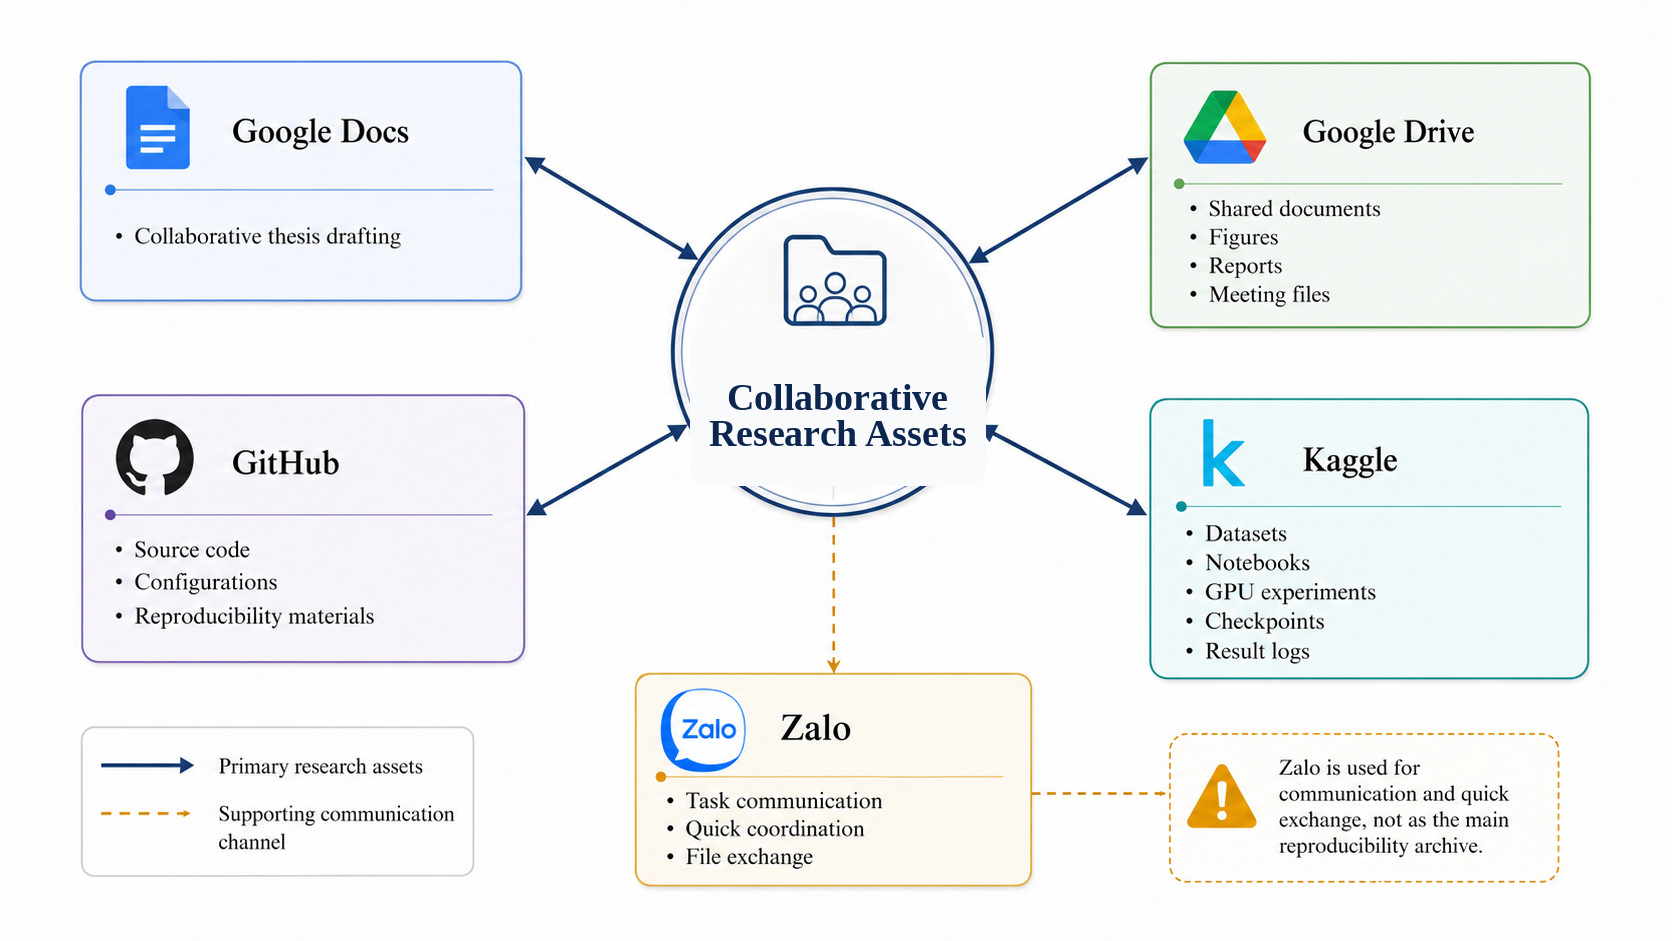
\includegraphics[width=0.94\textwidth,height=0.62\textheight,keepaspectratio]{assets/chapters_1_2/figure_2_5_artifact_flow.png}
\caption{Document and experiment artifact flow.}
\end{figure}
The distinction between primary assets and communication is a quality-control requirement. Zalo may be used for quick file exchange, but final reproducibility evidence must be retained in structured repositories such as GitHub, Google Drive, or Kaggle rather than relying on chat history alone.\par
\subsubsection{Dataset and Annotation Quality Assurance}
Dataset quality begins with source verification, class-count inspection, file-format checks, duplicate and repeated-view analysis, and explicit partition manifests. Classification preprocessing is audited by class so that background removal does not silently delete files or change class counts. External datasets are mapped with documented class semantics and split by source before partition-wise merging. These controls ensure that reported metrics can be related to known data rather than an undocumented folder state.\par
\rev{
Segmentation quality requires explicit label controls. BG and WSSV are the only positive mask classes. Healthy has no BG/WSSV polygon but remains in train, validation, and test as an empty-label negative. The 1,149 filename-compatible images are audited by specimen group; the 303 unmatched-name additions cannot be grouped and are tracked as an image-level stratified extension. Polygon correspondence, class semantics, and the single-annotator limitation remain explicit quality controls.
}
\subsubsection{Experimental and Model-Comparison Quality}
Classification comparisons are governed by a fixed seed-42 protocol, consistent image partitions, documented preprocessing, and a common evaluation script. Macro-F1 is the primary ranking measure because the four-class problem is imbalanced and includes a co-infection class. Accuracy, classwise scores, Kappa, parameters, size, latency, FPS, corruption results, and XAI may support interpretation, but they do not replace the declared primary selection rule.\par
\rev{
Direct segmentation baseline claims require the same grouped split, class mapping, mask format, image size, duration, seed, and evaluation settings. The CA-to-SimAM placement study is controlled across candidate insertion points. The broader attention-family comparison is not a strict one-factor ablation because archived runs differ in augmentation, epochs, software, initialization, placement, and auxiliary loss. Fourier variants use matched controls; qualitative panels supplement mask metrics with Healthy false positives, incomplete masks, merged regions, and difficult appearances.
}
protocol is controlled, and the evidence supports the stated contribution. A metric increase alone does not establish novelty. The thesis must distinguish adopted components, team modifications, reimplementations, and newly proposed combinations. Unsupported causal interpretations and claims that exceed the dataset or protocol are removed during quality review.\par
\subsubsection{Reproducibility and Artifact Quality}
Reproducibility quality connects every publishable number to a dataset version, split rule, seed, environment, configuration, evaluation command, checkpoint, and exported result. GitHub provides the structured source and documentation layer; Kaggle preserves executable notebooks and run outputs; Google Drive retains shared figures, documents, and packaged evidence. File exchange through Zalo is temporary and cannot be the only location of an accepted result.\par
Artifact review also checks internal consistency. The metric shown in a table must match the associated figure and discussion. Model names must not change meaning between methodology and results. Healthy must be described as a classification class and an empty-label segmentation negative, not as a segmentation mask class. ShrimpXNet must remain a literature reference for classification, whereas the proposed classification method is built directly on the selected YOLO26m-cls engineering baseline.\par
\subsubsection{Mobile and Document Quality}
\rev{
Mobile quality is assessed through Android flows and operational runtime, not production readiness. The common build always runs the FP32 classifier and conditionally dispatches the FP16 segmenter. Three Android devices provide branch-aware runtime under the same app/model configuration; image order is not standardized because the study targets runtime feasibility, not strict hardware ranking. The system remains a preliminary screening prototype.
}
Document quality is controlled at structural, visual, terminological, and evidential levels. Chapter numbering follows the official AIP491 template. Tables use consistent Times New Roman typography, page-safe widths, peach headers, centered cell text, and explanatory prose. Figures appear in the relevant subsection with captions and interpretation. Cross-references, abbreviations, dataset names, model names, dates, limitations, and final metrics are checked before submission.\par
\subsection{Budget and Funding (Optional)}
No direct project budget was incurred. The team used public datasets, open-source frameworks, free Kaggle Notebook GPU allocations, existing Android devices, Firebase free-tier services, institutional resources, and no-cost collaboration tools. The table documents the resource model without inventing monetary expenditure.\par
\begingroup
\CVioTableSetup
\begin{longtable}{|>{\centering\arraybackslash}p{3.28cm}|>{\centering\arraybackslash}p{6.81cm}|>{\centering\arraybackslash}p{3.89cm}|}
\caption{Project resources and funding status}\\
\hline
\CVioPeachHeader\textbf{Resource category} & \textbf{Resource / funding source} & \textbf{Recorded cost status} \\ \hline
\endfirsthead
\caption[]{Project resources and funding status (continued)}\\
\hline
\CVioPeachHeader\textbf{Resource category} & \textbf{Resource / funding source} & \textbf{Recorded cost status} \\ \hline
\endhead
\hline
\multicolumn{3}{r}{\footnotesize Continued on next page}\\
\endfoot
\hline
\endlastfoot
Datasets & ShrimpDiseaseImageBD and ShrimpDB public sources & No direct cost \\ \hline
Model development & Python, PyTorch, TorchVision, Ultralytics, OpenCV & Open source \\ \hline
GPU experiments & Kaggle Notebook; up to 2 $\times$ NVIDIA Tesla T4 when available & Free allocation \\ \hline
Mobile development & Android Studio, Kotlin, Java interoperability, TensorFlow Lite & Open source / existing equipment \\ \hline
Application data services & Firebase free-tier services & No recorded direct cost \\ \hline
Version control and collaboration & GitHub, Google Drive, Google Docs, Google Meet, Zalo & No recorded direct cost \\ \hline
Testing devices & Existing personal Android devices & No dedicated purchase \\ \hline
\end{longtable}
\endgroup
\subsubsection{Resource-Utilization Model}
The absence of a direct monetary budget does not mean the project has no resource plan. The team relies on public datasets, open-source libraries, free Kaggle GPU allocation, existing Android devices, Firebase free-tier services, university supervision, and no-cost collaboration platforms. These resources define the feasible model scale, experiment count, deployment approach, and schedule. The approximate sub-15M-parameter selection constraint is consistent with the mobile-oriented objective and the available deployment environment.\par
Compute is managed as a scarce shared resource. Baseline screening is used to narrow the candidate set before expensive improvement experiments. Failed or exploratory runs are first debugged at smaller scale when possible. Checkpoints and logs are preserved to avoid unnecessary repetition. Late-stage compute is reserved for matched comparisons, ablations, robustness, external evaluation, and the final evidence package rather than unlimited architecture search.\par
\subsubsection{Cost Control and Reporting Boundaries}
The project does not invent estimated prices for tools that were used without recorded payment. Open-source software is recorded as open source, free-tier services as no recorded direct cost, and existing devices as existing equipment. This reporting boundary avoids presenting an artificial financial analysis that cannot be verified. It also distinguishes direct expenditure from the non-monetary cost represented by member effort and experiment duration.\par
Resource changes are reviewed when they affect scientific comparability or delivery. Moving from one GPU environment to another, changing image size to fit memory, reducing epoch count, or replacing a mobile model format may alter the result and therefore cannot be treated only as a budget decision. The effect on protocol, schedule, and thesis interpretation must be assessed through change management.\par
\subsubsection{Sustainability and Maintainability of Resources}
The selected toolchain supports continuation after the capstone because it is based primarily on widely used open-source frameworks and accessible platforms. Source code and documentation can remain in GitHub, experiment notebooks can be rerun on compatible environments, and the Android application can be maintained without a proprietary inference runtime. Firebase free-tier dependence is documented so that future scaling or policy changes are not overlooked.\par
Sustainability also depends on preserving knowledge, not only files. The final repository and thesis should explain dataset preparation, class semantics, split construction, model selection, proposed modules, evaluation commands, mobile class order, known limitations, and artifact locations. A future maintainer should not need private chat history to determine how the accepted result was produced.\par
\subsection{Change Management Process}
A change may be triggered by council feedback, supervisor direction, experimental evidence, a technical blocker, dataset findings, deployment constraints, or document review. The team does not apply changes informally when they affect scope, comparison validity, dependencies, or reported conclusions. The impact is discussed, the decision is recorded, and accepted changes are reflected in tasks, dates, deliverables, experiments, and thesis wording.\par
Figure 2.5 presents the controlled path from a change trigger to documentation. Impact assessment considers scope, schedule, dependencies, and evaluation implications before the supervisor and team accept or revise the proposal.\par
\begin{figure}[tbp]
\centering
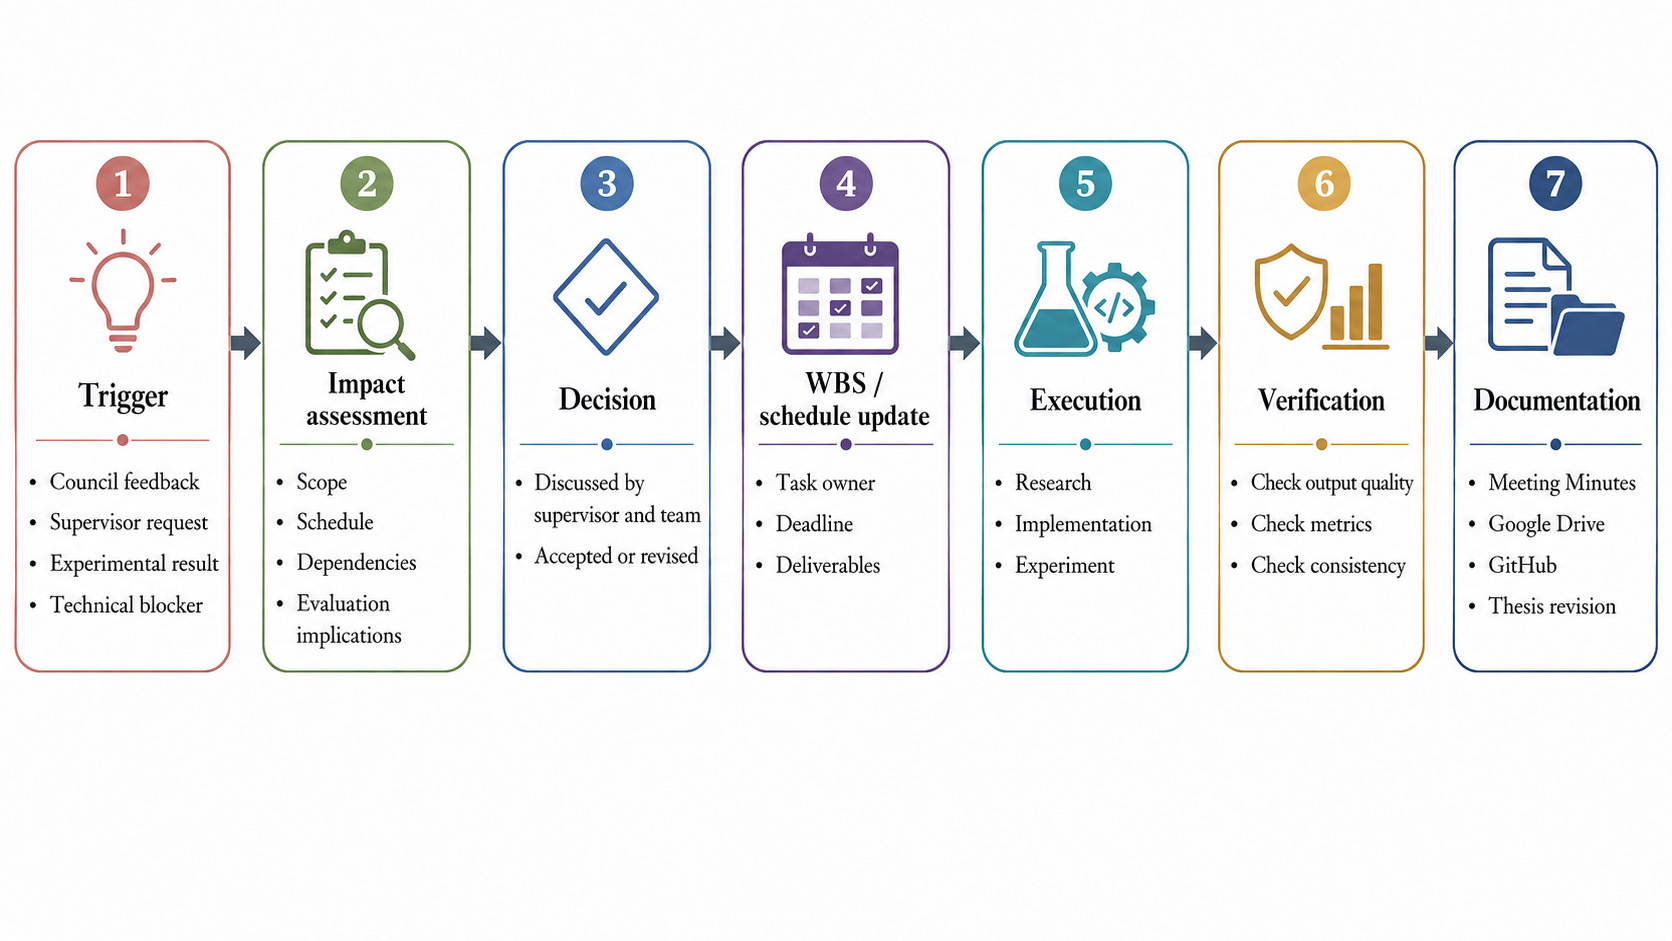
\includegraphics[width=0.94\textwidth,height=0.62\textheight,keepaspectratio]{assets/chapters_1_2/figure_2_6_change_process.jpeg}
\caption{Controlled change-management process.}
\end{figure}
\begingroup
\CVioTableSetup
\begin{longtable}{|>{\centering\arraybackslash}p{3.54cm}|>{\centering\arraybackslash}p{5.04cm}|>{\centering\arraybackslash}p{5.40cm}|}
\caption{Change categories and control requirements}\\
\hline
\CVioPeachHeader\textbf{Change category} & \textbf{Assessment criterion} & \textbf{Required control} \\ \hline
\endfirsthead
\caption[]{Change categories and control requirements (continued)}\\
\hline
\CVioPeachHeader\textbf{Change category} & \textbf{Assessment criterion} & \textbf{Required control} \\ \hline
\endhead
\hline
\multicolumn{3}{r}{\footnotesize Continued on next page}\\
\endfoot
\hline
\endlastfoot
Minor implementation change & Does not alter dataset, split, metric, architecture claim, or deadline & Project leader coordinates and records the update \\ \hline
Experimental protocol change & Affects preprocessing, augmentation, seed, checkpoint selection, metric, or evaluation & Supervisor and team review before results are treated as comparable \\ \hline
Scope extension & Adds a formal research track, dataset, application function, or deliverable & Discuss impact; update WBS, schedule, ownership, and thesis scope \\ \hline
Schedule change & Moves a milestone or depends on unfinished GPU, labeling, or integration work & Update responsible owner and revised deadline during review \\ \hline
Document interpretation change & Changes the meaning of baseline, proposed result, limitation, or contribution & Verify evidence and apply consistently across methodology, results, discussion, and conclusion \\ \hline
\end{longtable}
\endgroup
\subsubsection{Change Initiation and Classification}
A change is initiated when new information makes the current plan incomplete, invalid, or inefficient. Triggers include council feedback, supervisor direction, experimental evidence, dataset findings, implementation failure, deployment constraints, dependency delays, or document review. The initiator states what must change, why the current state is insufficient, and which workstreams or conclusions may be affected.\par
Changes are classified by impact. A minor implementation correction does not alter the dataset, protocol, architecture claim, metric, or deadline. An experimental-protocol change affects comparability and requires review before new and old results are placed in the same table. A scope extension adds a formal track, dataset, function, or deliverable. A schedule change moves a milestone or dependency. A document-interpretation change alters the meaning of a baseline, proposed result, limitation, or contribution and therefore requires evidence verification.\par
\subsubsection{Impact Assessment and Decision}
Impact assessment examines scope, owner workload, dataset requirements, implementation effort, GPU time, dependencies, mobile effects, documentation changes, and the validity of previously produced evidence. The team determines whether earlier work remains usable, must be rerun, or needs to be relabeled. A proposed change is accepted only when its value and required work are understood; otherwise it is revised, postponed, or rejected.\par
\rev{
Earlier review feedback triggered the instance-segmentation scope extension; responsibilities, WBS items, and thesis sections were updated accordingly. The later Council No. 03 post-defense revision is recorded separately in Section 2.5.5.
}
The supervisor has the strongest role when a change affects research direction, contribution, evaluation protocol, or milestone acceptance. The project leader coordinates the operational update and checks cross-workstream effects. The responsible technical member estimates implementation and evidence requirements. This distribution prevents a local code change from silently becoming a new scientific claim.\par
\subsubsection{Implementation, Verification, and Documentation}
An accepted change is translated into revised tasks, owners, dates, dependencies, outputs, and acceptance conditions. Implementation then follows the same research sequence as other work: investigate, implement, experiment, evaluate, and review. Verification checks whether the change solved the initiating problem and whether it introduced a new inconsistency. The result is documented in Meeting Minutes, the WBS or schedule where relevant, structured artifact stores, and the thesis.\par
The addition of instance segmentation demonstrates the complete process. Council feedback identified insufficient research depth in the initial classification-only scope. The team accepted a formal segmentation track, defined mask-annotation work, assigned attention and mobile work to Nhu, assigned annotation, grouped split, leakage, and Fourier work to Phong, retained classification ownership with Nhan, and updated the final system and thesis scope. Later grouped splitting further refined the segmentation protocol after repeated-specimen concerns were identified.\par
\subsubsection{Cross-Document Consistency Control}
A change is incomplete if only one paragraph is updated. Scope changes must be reflected in the introduction, objectives, methodology, results, project plan, figures, limitations, conclusion, WBS, Gantt chart, and role descriptions where applicable. Experimental changes must update configuration descriptions, table labels, metric interpretation, and reproducibility artifacts. Terminology changes must be propagated consistently to prevent conflicting automated or human readings of the thesis.\par
\rev{
Before final acceptance, the project leader audits high-risk terms and values: YOLO26m-cls selection, ASL-LDAM/SimAM-DCFR naming, the locked 91.01\% Macro-F1, Healthy segmentation semantics, split boundaries, attention/Fourier interpretation, two-model dispatch, runtime provenance, external-data limits, and non-clinical use. This links change management directly to document quality.
}
\subsubsection{\rev{Post-Defense Council Revision Cycle}}
\rev{
The 5 August 2026 DOCX package is retained as the initial pre-defense submission freeze. Council No. 03 reviewed the project on 9 August 2026 and required mandatory revisions before 12:00 on 15 August 2026. This post-defense cycle is treated as a controlled change extension rather than a retroactive rewrite of the historical WBS and Gantt chart. Accepted work includes additional component and comparator evidence, Fourier-spectrum analysis, final two-model mobile documentation, three-device Android runtime evidence, real-world three-camera operational evidence, and response-letter traceability.
}
\subsection{\rev{Closure and Evaluation}}
\rev{
Project closure uses the revised-submission gate rather than the initial defense freeze. The initial DOCX was submitted on 5 August 2026; Council No. 03 issued revision requirements on 9 August; and the controlled revision is due before 12:00 on 15 August 2026. Closure requires evidence, reproducibility, application functionality, document consistency, response-letter traceability, and archive completeness.
}
\begingroup
\CVioTableSetup
\begin{longtable}{|>{\centering\arraybackslash}p{3.89cm}|>{\centering\arraybackslash}p{10.08cm}|}
\caption{Project closure and Definition of Done}\\
\hline
\CVioPeachHeader\textbf{Closure criterion} & \textbf{Definition of Done} \\ \hline
\endfirsthead
\caption[]{Project closure and Definition of Done (continued)}\\
\hline
\CVioPeachHeader\textbf{Closure criterion} & \textbf{Definition of Done} \\ \hline
\endhead
\hline
\multicolumn{2}{r}{\footnotesize Continued on next page}\\
\endfoot
\hline
\endlastfoot
Classification research complete & The final proposed classifier is fully specified; Macro-F1 is reported consistently as 91.01\%; clean and corruption comparisons are traceable; component-evidence wording is internally consistent. \\ \hline
\rev{Segmentation research complete} & \rev{BG/WSSV labels, Healthy empty-label handling, the specimen-grouped 1,149-image subset, the unmatched-name expansion boundary, baselines, attention/Fourier evidence, metrics, qualitative analysis, and limitations are documented.} \\ \hline
Improvement criterion satisfied & Each claimed proposed method is compared against the relevant controlled baseline and is supported by the declared metric and evidence. \\ \hline
Research novelty documented & The thesis clearly identifies what is adopted, reimplemented, modified, or newly proposed; unsupported novelty claims are removed. \\ \hline
Reproducibility package complete & Datasets, split rules, seed, environment, configurations, code, checkpoints, logs, metrics, figures, and model metadata are archived. \\ \hline
\rev{Mobile prototype complete} & \rev{One common Android application/model configuration executes the FP32 classifier for every accepted image and conditionally invokes the FP16 segmenter; branch-aware operational runtime from three Android devices is archived without claiming field accuracy or iOS support.} \\ \hline
Paper and thesis complete & Classification paper material, segmentation documentation, tables, figures, references, limitations, and conclusions are integrated and reviewed. \\ \hline
\rev{Final quality audit complete} & \rev{Section numbering, A4 page geometry, Times New Roman typography, table/figure placement, yellow revision highlighting, terminology, metrics, dates, limitations, and cross-document consistency pass the final rendered audit.} \\ \hline
Defense preparation complete & Presentation content, demonstration path, role allocation, likely questions, and evidence references are prepared. \\ \hline
\rev{Final submission complete} & \rev{The 5 August initial defense package and the Council-mandated revised package due before 12:00 on 15 August 2026 are both traceable; accepted artifacts are archived.} \\ \hline
\end{longtable}
\endgroup
\rev{
Table 2.11 defines closure by evidence, reproducibility, functional integration, and academic consistency. The 5 August package remains historical; closure requires the Council-mandated revision and final audit.
}
\subsubsection{\rev{Closure Readiness Review}}
\rev{
Closure readiness is assessed against the revised 15 August 2026 submission gate. Each workstream confirms that required outputs are available, accepted limitations are stated, unresolved placeholders are removed, and cross-workstream dependencies have been integrated. Classification, segmentation, mobile, documentation, reproducibility, response-letter evidence, and defense revisions are reviewed as connected components of one project; a missing artifact in one component can prevent closure even when another component has a strong metric.
}
\rev{
The readiness review distinguishes mandatory corrections from desirable extensions. Mandatory work includes the Council-requested evidence, controlled baseline/proposed comparisons, split and mask documentation, two-model mobile integration, traceable runtime reporting, template-compliant chapters, consistent figures and tables, references, limitations, and the revised DOCX/PDF package. Additional experiments are accepted only when they can be completed and integrated without destabilizing the required revision.
}
\subsubsection{\rev{Final Scientific and Reproducibility Audit}}
\rev{
The scientific audit checks whether every main claim is supported by the declared protocol and whether the scope of interpretation matches the evidence. It verifies the YOLO26m-cls deployment-oriented selection rationale, component evidence, multi-source retraining boundary, Healthy segmentation semantics, original-versus-expanded split validity, YOLO11n-seg selection trade-off, attention placement study, Fourier-spectrum analysis, three-device Android runtime interpretation, qualitative real-world evidence, and external-validation limits. Unsupported real-time, clinical, causal, iOS, field-accuracy, or universal-generalization claims are removed.
}
\rev{
The reproducibility audit checks dataset references, split construction, seed, training environment, configurations, checkpoint identity, evaluation scripts, result files, figures, tables, model artifacts, application build information, and repository documentation. Training on dual NVIDIA Tesla T4, notebook/GPU efficiency measurements, and Android application-recorded runtime are treated as three separate provenance categories and are not numerically conflated.
}
\subsubsection{\rev{Artifact Handover and Project Continuity}}
\rev{
Project handover is organized around structured assets. GitHub retains maintainable code and reproducibility documentation; Kaggle retains permitted datasets, notebooks, checkpoints, and run outputs; Google Drive retains the integrated thesis, figures, meeting records, response materials, and packaged evidence. The Android application, final FP32 classification artifact, final FP16 segmentation artifact, Firebase configuration documentation, device/runtime evidence, and presentation material are retained with the final archive. Zalo remains communication history rather than the authoritative research repository.
}
\rev{
Continuity information includes the conditions under which the accepted evidence remains valid. Future teams must know that segmentation masks were created by one annotator, Healthy is an empty-label segmentation negative rather than a mask class, specimen grouping is enforceable only where compatible filename structure exposes specimen identity, external data remain limited, background removal is classification-specific, and mobile runtime is device- and branch-dependent. The real-world photographs do not carry veterinary or laboratory disease ground truth, and the revised study does not establish iOS support.
}
\subsubsection{\rev{Lessons Learned and Final Evaluation}}
\rev{
The main management lesson is that AI research requires continuous alignment between data, implementation, evaluation, deployment, and documentation. A model result cannot be managed independently from the split that produced it, the checkpoint that was selected, the evaluation code that interpreted it, or the claim that appears in the thesis. Weekly evidence review, explicit task ownership, structured artifact storage, and controlled scope changes were therefore more useful than adopting a nominal software process that the team did not actually practice.
}
\rev{
A second lesson is that scope expansion must be accompanied by resource and validity controls. Adding instance segmentation increased research depth but introduced annotation semantics, single-annotator limitations, repeated-specimen leakage risk, attention/Fourier comparison boundaries, conditional mobile execution, and additional documentation. The post-defense Council revision reinforced the same principle: new evidence is useful only when its provenance, comparison limits, and cross-document consequences are controlled.
}
\rev{
Final evaluation combines scientific, engineering, and academic criteria. The classification and segmentation contributions must be supported against their relevant baselines under declared protocols; the Android application must demonstrate the approved conditional two-model functions; runtime evidence must remain branch-aware and non-clinical; reproducibility artifacts must be traceable; and the final thesis must communicate results, limitations, dates, and scope consistently. The 5 August 2026 package is the initial defense submission, while successful completion of the Council-mandated revision before 12:00 on 15 August 2026 constitutes the revised project-closure gate.
}
